% ====================================================================
% VİZE RAPOR ŞABLONU – Türk Masalları Derlemesi Web Sayfası
% --------------------------------------------------------------------
% DERLEME: Overleaf'te Menu > Compiler > XeLaTeX (pdfLaTeX de çalışır).
%
% KURALLAR (şablonu kullanmadan önce okuyun):
%  1. Bölüm başlıklarını SİLMEYİN ve sırasını DEĞİŞTİRMEYİN.
%  2. [KÖŞELİ PARANTEZ] içindeki ve gri renkli açıklama metinlerini
%     kendi bilgilerinizle değiştirin; açıklama metinlerini silin.
%  3. MEBİS'e YALNIZCA bu raporun PDF'ini yükleyin.
%     ZIP ve HTML dosyası YÜKLEMEYİN. Tüm kontroller GitHub'dan yapılır.
%  4. Kapaktaki GitHub ve YouTube bağlantıları doğru ve tıklanabilir
%     olmalıdır. Teslimden önce PDF'teki bağlantılara tıklayıp deneyin.
%  5. Haftalık katkı tablosundaki görseller için resim dosyalarını
%     (hafta1.png, hafta2.png, ...) Overleaf projesine yükleyin.
%     Dosya adlarında boşluk ve Türkçe karakter kullanmayın.
%     Resim yoksa tabloda "görsel ekleyin" kutusu görünür.
%  6. Yapay zekâ kullandıysanız Bölüm 5'i doldurun.
% ====================================================================
\documentclass[12pt,a4paper]{article}

\usepackage{iftex}
\ifPDFTeX
  \usepackage[T1]{fontenc}
  \usepackage[utf8]{inputenc}
\else
  \usepackage{fontspec}
\fi
\usepackage[provide=*,turkish]{babel}
\usepackage[margin=2.4cm]{geometry}
\usepackage{setspace}
\usepackage{graphicx}
\usepackage{booktabs}
\usepackage{longtable}
\usepackage{array}
\usepackage{colortbl}
\usepackage{xcolor}
\usepackage{enumitem}
\usepackage{listings}
\usepackage{amssymb}
\usepackage{caption}
\usepackage{fancyhdr}
\usepackage{hyperref}

\onehalfspacing
\setlength{\parindent}{0pt}
\setlength{\parskip}{6pt}
\setlength{\headheight}{15pt}
\setlength{\emergencystretch}{2em}
\setlist{itemsep=2pt, topsep=4pt}
\hypersetup{colorlinks=true, linkcolor=blue!50!black, urlcolor=blue!50!black}

\definecolor{ana}{HTML}{14325C}
\definecolor{acik}{HTML}{EEF2F8}

\lstset{basicstyle=\ttfamily\small, backgroundcolor=\color{acik},
  frame=single, rulecolor=\color{ana}, breaklines=true,
  columns=fullflexible, keepspaces=true, showstringspaces=false}

\pagestyle{fancy}
\fancyhf{}
\fancyhead[L]{Bir Varmış Bir Yokmuş}
\fancyhead[R]{Vize Raporu}
\fancyfoot[C]{\thepage}

% ---------- Yardımcı komutlar ----------
% Gri açıklama metni (silinecek yönergeler için)
\newcommand{\aciklama}[1]{{\color{gray}\itshape (#1)}}

% Haftalık tablo görseli: dosya yoksa "görsel ekleyin" kutusu çıkar
\newcommand{\haftagorsel}[1]{%
  \IfFileExists{#1}{%
    \includegraphics[width=\linewidth,height=4.2cm,keepaspectratio]{#1}%
  }{%
    \fbox{\parbox[c][2.6cm][c]{\dimexpr\linewidth-2\fboxsep-2\fboxrule\relax}{%
      \centering\small\color{gray} Ekran görüntüsü / görsel ekleyin\\ \texttt{#1}}}%
  }%
}
% Haftalık katılım kutuları (işaretlemek için $\square$ yerine $\boxtimes$ yazın)
\newcommand{\katilimkutulari}{\par\vspace{3pt}\small $\square$ Ders içinde katılım sergiledim\par $\square$ Telafi yaptım}

% Ek görsel: dosya yoksa hiçbir şey göstermez
\newcommand{\haftaek}[1]{%
  \IfFileExists{#1}{\par\vspace{4pt}\includegraphics[width=\linewidth,height=4.2cm,keepaspectratio]{#1}}{}%
}

% ---------- Kapak bilgileri ----------
\newcommand{\universite}{İstanbul Medipol Üniversitesi\\Görsel İletişim Tasarımı Bölümü}
\newcommand{\dersadi}{Programlamaya Giriş}
\newcommand{\hocaadi}{Meral Şentürk}
\newcommand{\ogrenciadi}{Elif Ün}
\newcommand{\ogrencino}{86230054}
\newcommand{\projeadi}{Bir Varmış Bir Yokmuş}
% Bağlantıları tam adres olarak yazın (https:// ile başlayarak)
\newcommand{\githublink}{\url{https://github.com/Elifunn/elifunprogramlamayagairis}}
\newcommand{\youtubelink}{\url{https://www.youtube.com/watch?v=Vbze7OP_Z9A}}


\newcommand{\derskatilimi}{\par\vspace{3pt}\small $\boxtimes$ Ders içinde katılım sergiledim\par $\square$ Telafi yaptım}
\newcommand{\telafikatilimi}{\par\vspace{3pt}\small $\square$ Ders içinde katılım sergiledim\par $\boxtimes$ Telafi yaptım}

\begin{document}

% ====================================================================
% KAPAK
% ====================================================================
\begin{titlepage}
\centering
\vspace*{1cm}
{\large \universite \par}
\vspace{1.8cm}
{\Huge\bfseries\color{ana} \projeadi \par}
\vspace{0.4cm}
{\Large Türk Masalları Derlemesi Web Sayfası \par}
{\large Vize Raporu \par}
\vspace{1.8cm}
{\large \textbf{Ders:} \dersadi \par}
{\large \textbf{Öğretim Üyesi:} \hocaadi \par}
\vspace{1.2cm}
{\large \textbf{Hazırlayan:} \ogrenciadi \par}
{\large \textbf{Öğrenci No:} \ogrencino \par}
\vspace{1.8cm}
\fbox{\parbox{0.88\linewidth}{\centering\vspace{6pt}
{\large\bfseries Proje Bağlantıları}\\[8pt]
\textbf{GitHub deposu:}\\ \githublink \\[8pt]
\textbf{YouTube sunum videosu:}\\ \youtubelink
\vspace{6pt}}}
\vfill
{\large \today \par}
\end{titlepage}

\tableofcontents
\newpage

% ====================================================================
\section{Giriş}
% ====================================================================


\subsection{Proje Özeti}
“Bir Varmış Bir Yokmuş”, Programlamaya Giriş dersi kapsamında hazırlanan bir Türk masalları derlemesi web sayfasıdır. Proje, farklı temalara sahip sekiz masalı ortak bir okuma ortamında bir araya getirmektedir. Kullanıcı masal başlıklarına göre arama yapabilmekte ve seçtiği masalı ayrı bir okuma alanında görüntüleyebilmektedir. Okuma alanının açık ve koyu renk seçenekleri bulunmaktadır. Lacivert ve altın renk paleti geceyi ve masalsı bir atmosferi çağrıştırmaktadır. İndirilebilir sürüm, içsel CSS ve JavaScript kodlarını barındıran tek bir HTML dosyasından oluşmaktadır. Sayfa internetsiz çalışmakta ve telefonda açılmaktadır. Rapor; masal seçimlerini, tasarım kararlarını, kodun çalışma mantığını ve haftalık katkıları açıklamaktadır.

\subsection{Gereksinimlerin Karşılanması}
\begin{center}
\rowcolors{2}{acik}{white}
\begin{tabular}{@{}p{8.2cm}c@{}}
\toprule
\rowcolor{ana}\textcolor{white}{\textbf{Gereksinim}} & \textcolor{white}{\textbf{Durum}} \\
\midrule
Masal sayısı 8--12 arasında (8 masal)         & $\boxtimes$ \\
Tek HTML dosyası                                    & $\boxtimes$ \\
Stil kodları içsel (\texttt{<style>} içinde)        & $\boxtimes$ \\
Betik kodları içsel (\texttt{<script>} içinde)      & $\boxtimes$ \\
İnternetsiz açılıp çalışıyor                        & $\boxtimes$ \\
JavaScript sayfada anlamlı bir işlev görüyor        & $\boxtimes$ \\
Sayfa telefonda da düzgün görünüyor                 & $\boxtimes$ \\
\bottomrule
\end{tabular}
\end{center}


% ====================================================================
\section{Masalların Seçimi}
Masal seçiminde, araştırma sırasında ilgi çeken olay örgüleri ve farklı temaların aynı seçkide bulunması belirleyicidir. Sevginin değerini anlama, iyilik, nankörlük ve sorumluluk gibi konular seçkinin temelini oluşturmaktadır. Tablodaki tür ifadeleri anlatıların genel özelliklerini tanımlar. Metinler kaynaklara dayalı kısaltılmış anlatımlardır.

% ====================================================================


\begin{longtable}{@{}cp{4cm}p{3cm}p{5.4cm}@{}}
\toprule
\textbf{No} & \textbf{Masal} & \textbf{Tür} & \textbf{Seçilme nedeni} \\
\midrule
\endhead
1 & Keloğlan ve Altın Bülbül & Olağanüstü masal & Yolculuk, yardım ve kardeşler arasındaki kıskançlığı birlikte işlemesi. \\[4pt]
2 & Ali Cengiz Oyunu & Olağanüstü masal & Biçim değiştirme ve zekâyla mücadele etme unsurları. \\[4pt]
3 & Nardaniye Hanım & Olağanüstü masal & Kıskançlık ve haksızlık karşısında gerçeğin ortaya çıkması. \\[4pt]
4 & Tuz Kadar Sevgi & Halk masalı & Sıradan görünen bir şeyin değerinin yokluğunda anlaşılması. \\[4pt]
5 & Üç Turunçlar & Olağanüstü masal & Büyülü meyveler, dönüşümler ve arayış teması. \\[4pt]
6 & Kırkıncı Oda & Olağanüstü masal & Bir hatanın sorumluluğunu üstlenme ve sonuçlarını düzeltme çabası. \\[4pt]
7 & Korkak Adam ve Devler & Mizahi ve olağanüstü masal & Korku ve kurnazlığın mizahi karşılaşmalarla anlatılması. \\[4pt]
8 & Değirmenci ile Tilki & Hayvan figürlü halk masalı & Yapılan iyiliğin unutulması ve nankörlük konusu. \\[4pt]
\bottomrule
\end{longtable}

% ====================================================================
\section{Tasarım Kararları}
% ====================================================================


\subsection{Konuya Uygunluk}
Sayfanın görsel yaklaşımı gece ve masal kavramlarına dayanmaktadır. Lacivert zemin gece atmosferini, altın tonları masalsı anlatımı desteklemektedir. “Bir varmış, bir yokmuş” başlığı masal temasını girişte belirtmektedir. Krem okuma alanı kitap sayfasını çağrıştırmakta ve metni kart listesinden ayırmaktadır. Görsel kalabalık yerine tipografi, boşluk ve renk karşıtlığı öne çıkmaktadır.

\subsection{Renk Paleti ve Yazı Tipi}
\begin{center}
\rowcolors{2}{acik}{white}
\begin{tabular}{@{}llp{6.4cm}@{}}
\toprule
\rowcolor{ana}\textcolor{white}{\textbf{Ad}} & \textcolor{white}{\textbf{Kod}} & \textcolor{white}{\textbf{Nerede / neden kullandınız?}} \\
\midrule
Lacivert & \texttt{\#101B30} & Ana zeminde gece atmosferi. \\
Altın & \texttt{\#DFBB75} & Başlık, numara ve düğmelerde vurgu. \\
Koyu mavi & \texttt{\#192842} & Kartlar ve koyu okuma görünümü. \\
Krem & \texttt{\#F5F0E6} & Yazılar ve açık okuma zemini. \\
Georgia & -- & Başlıklarda klasik kitap görünümü. \\
Arial & -- & Metinlerde sade, okunabilir görünüm. \\
\bottomrule
\end{tabular}
\end{center}

\subsection{Okunabilirlik, Gezinme ve Duyarlı Tasarım}
\begin{itemize}
  \item \textbf{Okunabilirlik:} Başlıklar ve açıklamalarda farklı büyüklükler kullanılır. Genel satır yüksekliği 1.7, okuma paragraflarının en fazla genişliği 680 pikseldir. Açık ve koyu yüzeylerde karşıt metin renkleri bulunur.
  \item \textbf{Gezinme:} Kartlardaki “Masalı oku” düğmesi okuma alanını açar. Arama kutusu başlığa göre listeyi daraltır. “Listeye dön” düğmesi okuma alanını kapatır.
  \item \textbf{Duyarlı tasarım:} Kartlar geniş ekranda üç sütun, 800 piksel ve altında iki sütun, 540 piksel ve altında tek sütundur. Dar ekranda başlık ve kenar boşlukları küçülür.
  \item \textbf{Tutarlılık:} Bütün kartlarda aynı numara, başlık, açıklama ve düğme düzeni kullanılır. Renkler ve boşluklar sayfa genelinde tutarlıdır.
\end{itemize}

\clearpage
\subsection{Ekran Görüntüleri}


\begin{figure}[htbp]
\centering
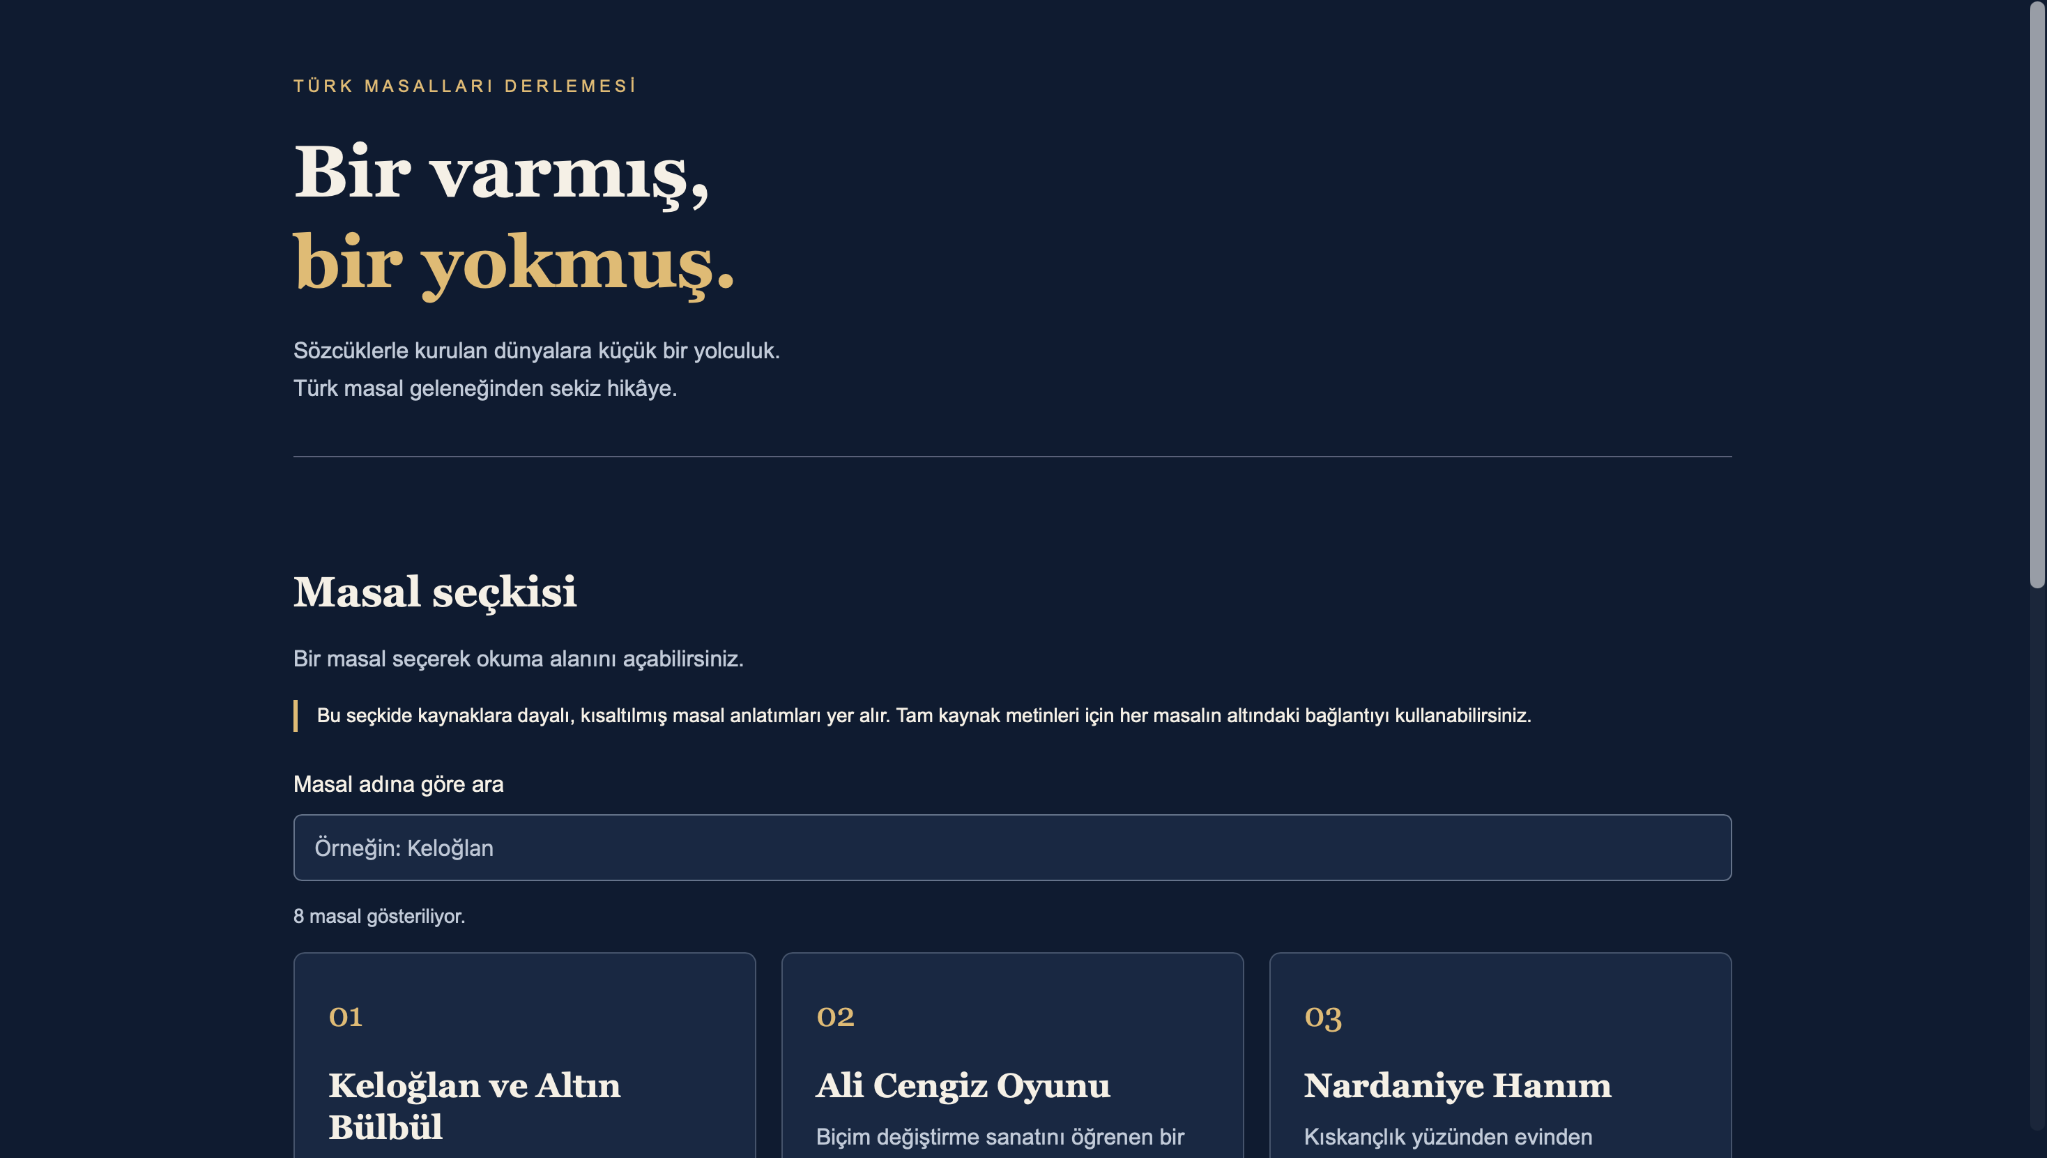
\includegraphics[width=0.9\textwidth]{ekran-masaustu.png}
\caption{Sayfanın bilgisayar görünümü}
\end{figure}
\begin{figure}[htbp]
\centering
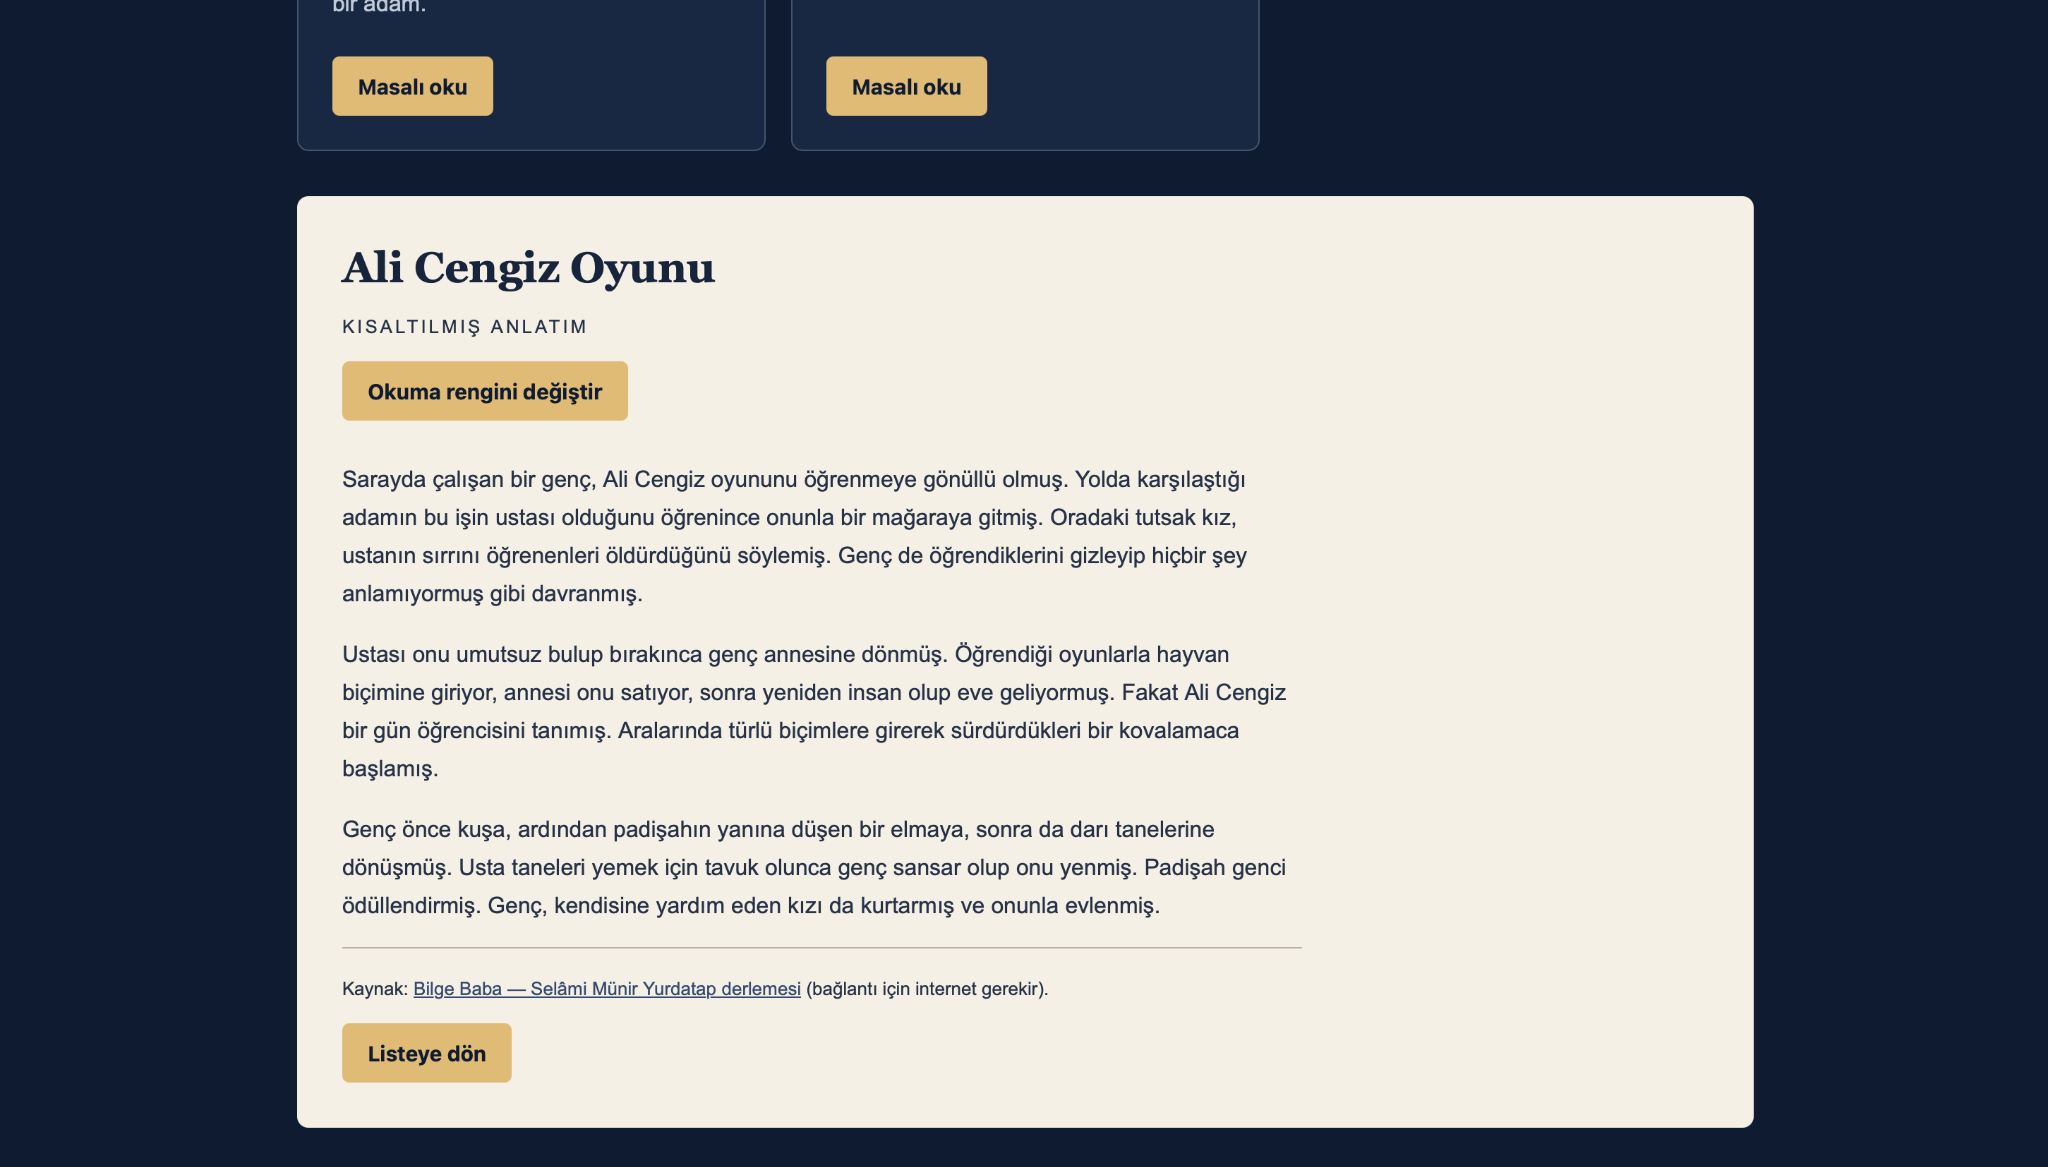
\includegraphics[width=0.9\textwidth]{ekran-okuma.png}
\caption{Masal okuma alanı ve renk değiştirme düğmesi}
\end{figure}
\clearpage
\section{Gerçekleştirme}
% ====================================================================


\subsection{HTML Yapısı}
Giriş bölümü \texttt{header}, ana içerik \texttt{main} etiketi içinde yer alır. Masal listesi bir \texttt{section} içinde, her masal ise \texttt{article} etiketiyle tanımlanan bir kartta bulunur. Kartlarda sıra numarası, \texttt{h3} başlığı, kısa açıklama ve okuma düğmesi vardır. Masal paragrafları \texttt{hikaye} sınıfına sahip alanlarda tutulur. \texttt{hidden} niteliği bu metinleri başlangıçta gizler. Sayfanın altındaki okuma alanı, seçilen masalın başlığını, metnini ve kaynak bağlantısını gösterir. Renk değiştirme ve listeye dönme düğmeleri bu alandadır.

\subsection{İçsel CSS}
Stil kodları, indirilebilir sürümde \texttt{style} etiketi içindedir. Grid, kart listesinin sütun düzenini oluşturur. Flex, kart içindeki öğeleri dikey sıralar. Düğmelerdeki \texttt{margin-top: auto}, düğmelerin alta yerleşmesini sağlar. \texttt{:hover} fareyle üzerine gelinen düğmenin rengini değiştirir. Medya sorguları ekran genişliğine göre sütun sayısını düzenler.

\begin{lstlisting}[caption={İçsel CSS'ten önemli bir bölüm}]
.masallar {
  display: grid;
  grid-template-columns: repeat(3, 1fr);
  gap: 18px;
}
@media (max-width: 800px) {
  .masallar { grid-template-columns: repeat(2, 1fr); }
}
@media (max-width: 540px) {
  .masallar { grid-template-columns: 1fr; }
}
\end{lstlisting}

\subsection{İçsel JavaScript}
Betik kodları HTML içeriğinin ardından \texttt{script} etiketi içinde bulunur. Kod, kartları ve okuma alanını seçer. Kart düğmelerine \texttt{addEventListener} ile tıklama olayı bağlar. Seçilen başlığı \texttt{textContent}, dosyadaki hazır masal içeriğini \texttt{innerHTML} üzerinden okuma alanına aktarır. Arama, Türkçe küçük harfe çevrilen başlıklarda \texttt{includes} ile eşleşme arar. Eşleşmeyen kartlar gizlenir ve sonuç sayısı güncellenir. Renk düğmesi, \texttt{classList.toggle} ile \texttt{gece} sınıfını ekleyip kaldırır. Renklerin kendisi CSS içinde tanımlıdır.

\begin{lstlisting}[caption={İçsel JavaScript'ten önemli bir bölüm}]
const renkDugmesi = document.getElementById("renk-degistir");
renkDugmesi.addEventListener("click", function () {
  const geceAcik = okuma.classList.toggle("gece");
  renkDugmesi.setAttribute("aria-pressed", geceAcik);
});
\end{lstlisting}

\subsection{Sayfanın Özellikleri}
\begin{itemize}
\item Sekiz masalı kartlar hâlinde listeleme ve başlığa göre arama.
\item Sonuç sayısını ve eşleşme bulunamadığında açıklama gösterme.
\item Seçilen masalı ayrı bir okuma alanında açma.
\item Okuma alanını açık ve koyu renkler arasında değiştirme.
\item Listeye dönme ve masal kaynaklarına bağlantı sunma.
\item Ekran genişliğine göre kartların sütun sayısını değiştirme.
\end{itemize}


% ====================================================================
\section{Yapay Zekâ Kullanımı}
% ====================================================================


\begin{longtable}{@{}p{2.6cm}p{3.6cm}p{4.2cm}p{3.4cm}@{}}
\toprule
\textbf{Araç} & \textbf{Ne için kullandınız?} & \textbf{İstem (prompt) özeti} & \textbf{Sayfada nerede?} \\
\midrule
\endhead
ChatGPT & Kod desteği & Sade, açıklanabilir HTML, CSS ve JavaScript kodları oluşturma. & Kartlar, arama ve okuma alanı. \\[5pt]
ChatGPT & Tasarım uygulaması & Lacivert-altın palet ve gece atmosferini kodla uygulama. & Zemin, başlıklar ve düğmeler. \\[5pt]
ChatGPT & Etkileşim & Dersteki renk değiştirme örneğini okuma alanına uyarlama. & Renk değiştirme düğmesi. \\[5pt]
ChatGPT & Metin ve açıklama & Kaynaklara dayalı kısa anlatımlar, kod açıklamaları ve rapor desteği. & Masal metinleri ve rapor. \\
\bottomrule
\end{longtable}

\subsection{Anladığım ve Kendim Yaptığım Kısımlar}
Kişisel katkılarım, masalların seçim gerekçeleri, lacivert-altın renk tercihi, gece atmosferi ve sade bir yapı talebidir. Kodların CodePen alanlarına yerleştirilmesi ve işlevlerin önizlemede denenmesi uygulama çalışmalarım arasındadır. Renk değiştirme düğmesi, dersteki örneğin okuma alanına uyarlanmasına dayanır. Ders adı ve yapay zekâ desteği bilgileri web sayfası yerine raporda yer almaktadır. HTML'in içerik yapısını, CSS'in görünümü, JavaScript'in etkileşimi oluşturduğunu kod üzerinden açıklayabilmekteyim.

% ====================================================================
\section{Haftalık Katkılar}
Haftalık çalışmalar, ders içi katılım ve telafi teslimleri olarak ayrılmıştır. Ekran görüntüsü dosyalarının çekim tarihleri ile çalışmanın ait olduğu ders haftası farklı olabilir; hafta eşleştirmesi çalışma ve teslim bilgilerine dayanmaktadır.

% ====================================================================


\begin{longtable}{@{}>{\raggedright\arraybackslash}p{1.7cm}%
                    >{\raggedright\arraybackslash}p{6.4cm}%
                    >{\centering\arraybackslash}p{6cm}@{}}
\toprule
\rowcolor{ana}\textcolor{white}{\textbf{Hafta}} & \textcolor{white}{\textbf{Yapılan çalışma}} & \textcolor{white}{\textbf{Görsel}} \\
\midrule
\endfirsthead
\toprule
\rowcolor{ana}\textcolor{white}{\textbf{Hafta}} & \textcolor{white}{\textbf{Yapılan çalışma}} & \textcolor{white}{\textbf{Görsel}} \\
\midrule
\endhead
\bottomrule
\endfoot

\textbf{1. hafta}\newline 16 Eylül &
Bu hafta için uygulama çalışmam bulunmamaktadır. Haftanın katılım değerlendirmesine dâhil olduğuna ilişkin doğrulanmış bilgi yoktur.\par\textbf{Commit:} Yok.\katilimkutulari &
Görsel kaydı bulunmamaktadır. \\
\midrule
\textbf{2. hafta}\newline 23 Eylül &
WorldWideWeb sayfası ders içi çalışmasıdır. Başlık, paragraf ve bağlantılarla içerik düzenini gösterir. Yazı tipi, renk, genişlik ve boşluk ayarları temel CSS kullanımını örneklendirir.\par\textbf{Commit:} Eşleştirme bulunmuyor.\derskatilimi &
\haftagorsel{hafta2.png} \\
\midrule
\textbf{3. hafta}\newline 30 Eylül &
Derin Denizler, Tıkla ve Galatasaray örnekleri telafi teslimidir. Çalışmalar görsel ve içerik düzenleme, düğmeyle uyarı açma ve fare olaylarıyla renk değiştirmeyi kapsamaktadır.\par\textbf{Commit:} Eşleştirme bulunmuyor.\telafikatilimi &
\haftagorsel{hafta3.png}
\haftaek{hafta3b.png}
\haftaek{hafta3c.png}
\haftaek{hafta3d.png} \\
\midrule
\textbf{4. hafta}\newline 7 Ekim &
Bu hafta için çalışma teslimi bulunmamaktadır. Tamamlanmış bir telafi kaydı da belirtilmemiştir.\par\textbf{Commit:} Yok.\katilimkutulari &
Görsel kaydı bulunmamaktadır. \\
\midrule
\textbf{5. hafta}\newline 14 Ekim &
Dört kartlı renk eşleme uygulaması ders içi çalışmasıdır. Tıklama, renk karşılaştırma ve eşleşen kartları gizleme işlemlerini içerir. Google'a bağlantı ve düğmeyle gitme örneği sayfa yönlendirmesini gösterir.\par\textbf{Commit:} Eşleştirme bulunmuyor.\derskatilimi &
\haftagorsel{hafta5.png}
\haftaek{hafta5b.png} \\
\midrule
\textbf{6. hafta}\newline 21 Ekim &
Merhaba sayfası ve turuncu kutunun rengini değiştirme uygulaması telafi teslimidir. Çağdaş Sanat ve Bienaller çalışması kendi teslim tarihinde yüklenen ödevdir. Örnekler harici CSS, anlamsal HTML ve düğmeyle stil değiştirmeyi kapsamaktadır.\par\textbf{Commit:} Eşleştirme bulunmuyor.\telafikatilimi &
\haftagorsel{hafta6.png}
\haftaek{hafta6b.png}
\haftaek{hafta6c.png}
\haftaek{hafta6d.png} \\
\midrule
\textbf{7. hafta} &
Bu raporda haftaya ait doğrulanmış çalışma ve katılım kaydı bulunmamaktadır.\par\textbf{Commit:} Belirtilmemiştir.\katilimkutulari &
Görsel kaydı bulunmamaktadır. \\
\midrule
\textbf{8. hafta} &
Bu raporda haftaya ait doğrulanmış çalışma ve katılım kaydı bulunmamaktadır.\par\textbf{Commit:} Belirtilmemiştir.\katilimkutulari &
Görsel kaydı bulunmamaktadır. \\
\end{longtable}

% ====================================================================
\section{Test ve Değerlendirme}
Bilgisayardaki CodePen önizlemesinde masal açma, arama, listeye dönme ve renk değiştirme işlevleri çalışmaktadır. İndirilebilir HTML dosyası internetsiz çalışmakta ve telefonda açılmaktadır. Kaynak sitelere yönlendiren bağlantılar internet gerektirmektedir. Başlıkta bir önizleme görüntüleme sorunu gözlemlenmiş, Chrome üzerinden incelemede başlık eksiksiz görünmüştür. Sorunun kesin nedeni belirlenmemiştir.

% ====================================================================


\begin{center}
\rowcolors{2}{acik}{white}
\begin{tabular}{@{}p{6cm}p{3.4cm}p{3.4cm}@{}}
\toprule
\rowcolor{ana}\textcolor{white}{\textbf{Özellik}} & \textcolor{white}{\textbf{Bilgisayar}} & \textcolor{white}{\textbf{Telefon}} \\
\midrule
Masalı açma ve listeye dönme & Çalışıyor & Ayrı işlev testi kaydı yok \\
Masal adına göre arama & Çalışıyor & Ayrı işlev testi kaydı yok \\
Okuma rengini değiştirme & Çalışıyor & Ayrı işlev testi kaydı yok \\
İnternetsiz kullanım & Çalışıyor & Ayrı test kaydı yok \\
Dosyanın açılması & Çalışıyor & Çalışıyor \\
\bottomrule
\end{tabular}
\end{center}

\textbf{Denenen tarayıcılar:} Chrome (başlık görünümü incelemesi). Kişisel işlev testlerinin tarayıcı adı ayrıca kaydedilmemiştir.

% ====================================================================
\section{Sunum Videosu}
% ====================================================================
\begin{center}
\begin{tabular}{@{}ll@{}}
\textbf{Video süresi:} & 20:47 \quad  \\
\textbf{Görünürlük:} & Hesap ayarı doğrulanmadı. \\
\textbf{Bağlantı:} & \youtubelink \\
\end{tabular}
\end{center}

Video süresi, 12--18 dakika koşulunun üst sınırını 2 dakika 47 saniye aşmaktadır. Boş kutular, ilgili koşulun karşılanmadığını veya bu rapor kapsamında doğrulanmadığını belirtmektedir.

\subsection{Video Kontrol Listesi}

\begin{itemize}[label={}]
  \item $\square$ Süre 12--18 dakika aralığında.
  \item $\square$ Sunum boyunca kameram açık, yüzüm görünüyor.
  \item $\square$ Görünürlük \textbf{Listelenmemiş} (ya da Herkese açık); \textbf{Özel} değil.
  \item $\square$ Bağlantıyı gizli pencerede açtım, video oynuyor.
  \item $\square$ YouTube videoyu işlemeyi bitirdi.
  \item $\square$ Videoyu baştan sona izledim; ses ve kamera tüm sunumda var.
  \item $\boxtimes$ Kapaktaki bağlantı ile bu bölümdeki bağlantı aynı.
\end{itemize}

% ====================================================================
\section{Sonuç ve Kendi Değerlendirmem}
% ====================================================================


Bu proje, HTML, CSS ve JavaScript'in farklı görevlerini uygulama üzerinden anlamamı sağlamıştır. İçerik, görünüm ve etkileşim arasındaki ilişki sayfanın bölümlerinde açık biçimde görülmektedir. Sade kod yapısı, bölümler arasındaki bağlantıyı takip etmemi kolaylaştırmıştır. CodePen önizlemesi, kod ile ekrandaki sonuç arasında ilişki kurmamı sağlamıştır. Farklı temalara sahip masallar ortak bir okuma ortamında buluşmaktadır. Renk değiştirme özelliği, dersteki bir çalışmanın başka bir amaca uyarlanmasını örneklendirmektedir. Yapay zekâ desteği kod geliştirme ve açıklama sürecine katkı sağlamıştır. Yazı büyüklüğü seçimi, projenin geliştirilebilecek özellikleri arasındadır.

% ====================================================================
\section{Kaynakça}
Kaynaklar, kısa masal anlatımlarının dayandığı çevrim içi metinleri gösterir. Derleme ve eser bilgileri ilgili kaynak sayfalardaki atıflardır; basılı eserlerin doğrudan incelendiği anlamına gelmez.

% ====================================================================


\begin{thebibliography}{9}
\bibitem{k1} Türkiye Kültür Portalı. \emph{Keloğlan ve Altın Bülbül Masalı}. Osman Saygı derlemesi. \url{https://kulturportali.gov.tr/portal/keloglanvealtinbulbulmasali}
\bibitem{k2} Bilge Baba. \emph{Ali Cengiz Oyunu}. Selâmi Münir Yurdatap derlemesi. \url{https://bilgebaba.com/alicengiz-oyunu}
\bibitem{k3} Bilge Baba. \emph{Nardaniye Hanım}. Pertev Naili Boratav, Zaman Zaman İçinde aktarımı. \url{https://bilgebaba.com/nardaniye-hanim}
\bibitem{k4} Masal Dergisi. \emph{Tuz Kadar Sevgi}. 2025, Sayı 28. \url{https://www.masaldergisi.com/sayilar/2025/sayi-28/tuz-kadar-sevgi/}
\bibitem{k5} Bilge Baba. \emph{Üç Turunçlar}. Nebahat Çetin derlemesi. \url{https://bilgebaba.com/uc-turunclar/}
\bibitem{k6} Okuryazar. \emph{Kırkıncı Oda}. Naki Tezel, Türk Masalları I aktarımı. \url{https://www.okuryazar.com.tr/dergi/kirkinci-oda}
\bibitem{k7} Türkiye Kültür Portalı. \emph{Korkak Adam ve Devler}. Salim Dalkıran derlemesi. \url{https://www.kulturportali.gov.tr/portal/korkakadamvedevler}
\bibitem{k8} Masal Sitesi. \emph{Değirmenci ile Tilki}.  \url{https://www.masalsitesi.com/Degirmenci-ile-Tilki-Masali.html}
\bibitem{k9} OpenAI. \emph{ChatGPT}. Kod, açıklama ve metin desteği; kapsamı Bölüm 5'tedir. \url{https://chatgpt.com/}
\end{thebibliography}

% ====================================================================
\appendix
\section{Teslim Kontrol Listesi}
% ====================================================================

\begin{itemize}[label={}]
  \item $\square$ MEBİS'e \textbf{yalnızca bu raporun PDF'ini} yükleyeceğim. ZIP ve HTML dosyası yüklemeyeceğim.
  \item $\boxtimes$ PDF dosya adı \texttt{86230054\_ElifUn\_vize.pdf} biçiminde.
  \item $\square$ Kapaktaki GitHub ve YouTube bağlantıları doğru; PDF'te tıklayıp denedim.
  \item $\square$ GitHub deposunda web sayfası (tek \texttt{.html}), rapor PDF'i, \texttt{.tex} kaynakları ve \texttt{README.md} var.
  \item $\square$ GitHub deposu \textbf{herkese açık} (ya da öğretim üyesine erişim verdim).
  \item $\square$ Çalışmamın son hâli teslim saatinden \textbf{önce} depoya gönderildi (sonraki commitler değerlendirilmez).
  \item $\boxtimes$ Sayfa içsel CSS ve içsel JavaScript kullanıyor, harici dosya gerektirmiyor.
  \item $\square$ Hazır taslak kullanmadım; yapay zekâ kullandıysam Bölüm 5'i doldurdum.
  \item $\square$ Çalışmanın mantığını sunumda anlatabilirim.
\end{itemize}

\end{document}